\chapter{Analysis of performance}

The execution time is measured and analyzed in detail.

\section{Variables of interest}

A simple test to determine the performance of the simulator is to measure the
time per iteration (using the wall clock). The time spent in the different
stages of the simulation can also be of interest.

Consider the sequence of time per iteration (also referred simply as the time)
$T_0,\ldots,T_n$ as independent random variables from a common distribution with
an unknown mean $\mu$ and finite standard deviation $\sigma$. The sample mean
$\overline T$ can be approximated with a certain degree of confidence by a
process of sampling.

Different parameters of the simulation may affect the time mean $\mu$ and is the
objective of this chapter to find out what the relation is. The time is at least
in $O(N_p)$, as we need to iterate over each particle $N_p$. We also know that
the worst-case complexity of the FFT is in $O(N_g \log N_g)$ for $N_g$ total grid
points.

The simulator runs for at least 30 iterations, and then the standard error of 
the mean (SEM) is computed. Then in each iteration is determined if the SEM is 
below a threshold to stop the simulation. The threshold is determined so that 
when the simulation stops, the mean is has an error of at most 0.2\% with 
probability 95\%.

\subsection{Number of particles}

The number of particles $N_p$ is one of the main parameters that affect the
running time of each iteration. In order to characterize the scalability of the
application, several tests are designed with increasing number of particles, and
different metrics are compared.

The wall clock is used in the process with rank zero to measure how long takes
each iteration.

\begin{figure}[h]
	\centering
	\subfloat[Increasing number of particles]{
		\begin{tikzpicture}
		\begin{axis}[
			width=0.5\textwidth,
			xlabel=Particles $N_p$,
			ylabel=Time per iteration (s),
			grid=major]
		\addplot [only marks,error bars/y dir=both, error bars/y explicit] table [
			x index = {0},
			y index = {3},
			y error index={4},
			col sep=space] {csv/particles.csv};
		\end{axis}
		\end{tikzpicture}
	}
	\subfloat[Increasing number of grid points]{
		\begin{tikzpicture}
		\begin{axis} [
			no markers,
			grid=major,
			xlabel=Grid points $N_g$,
			ylabel=Time per iteration (s),
			width=0.5\textwidth]
		\addplot [only marks,error bars/y dir=both, error bars/y explicit] table [
			x index = {0},
			y index = {3},
			y error index={4},
			col sep=space] {csv/solver.csv};
		\end{axis}
		\end{tikzpicture}
	}
	\caption{The effect of the variables $N_p$ and $N_g$ to the time per 
	iteration. Using one process and 32 CPUs (MPI communications are not needed).}
\end{figure}

\subsection{Constant number of CPUs}

The simulator is designed to scale with the number of particles when the number 
of CPUs or process are incremented, as each chunk can be computed in parallel.  
But when the number of grid points is incremented, the FFT solver must scale 
both in the number of CPUs and processes. The FFTW library offers two 
parallelization implementations for multithreading: Using OpenMP and POSIX 
threads (pthreads). OpenMP is not compatible with OmpSs-2 as we have one runtime 
already running so the pthread implementation was tested.
%
\begin{figure}[h]
	\centering
		\begin{tikzpicture}
		\begin{axis} [
			legend pos=north west,
			xmode=log,
			log basis x=2,
			xticklabels={0,1,2,4,8,16,32},
			grid=major,
			xlabel=Number of CPUs,
			ylabel=Time per iteration (s),
			width=10cm,
			height=6cm,
			]
		\addplot+ [only marks,error bars/y dir=both, error bars/y explicit] table [
			x index = {0},
			y index = {3},
			y error index={4},
			col sep=space] {csv/fftw-sequential.csv};
		\addlegendentry{Single thread}
		\addplot+ [only marks,error bars/y dir=both, error bars/y explicit] table [
			x index = {0},
			y index = {3},
			y error index={4},
			col sep=space] {csv/fftw-threads.csv};
		\addlegendentry{Multithread}
		\end{axis}
		\end{tikzpicture}
	\caption{The number of CPUs is increased with only one process: the solver 
	cannot scale and the time per iteration increases. Configuration used: $N_p = 
	\num{5e5}$, $N_g=8192\times8192$.}
	\label{fig:fftw-time}
\end{figure}
%
Unfortunately, the FFTW library doesn't show a good speedup, in fact worsens the 
time per iteration when adding more threads with the configurations tested. In 
the figure~\ref{fig:fftw-time} it can be shown how the time grows as the number 
of CPUs increases.
%
The FFTW documentation warns about this problem, claiming that it can only 
improve the time with large enough matrices:
%
\begin{displayquote}
A shared-memory machine is one in which all CPUs can directly access the same 
main memory, and such machines are now common due to the ubiquity of multi-core 
CPUs. FFTW’s multi-threading support allows you to utilize these additional CPUs 
transparently from a single program. However, this does not necessarily 
translate into performance gains---when multiple threads/CPUs are employed, 
there is an overhead required for synchronization that may outweigh the 
computational parallelism. Therefore, you can only benefit from threads if your 
problem is sufficiently large.
\end{displayquote}
%
However, larger matrices are not useful to get more precise results, as we 
rather prefer an increase in the number of particles than in grid points.


\begin{figure}[h]
	\centering
	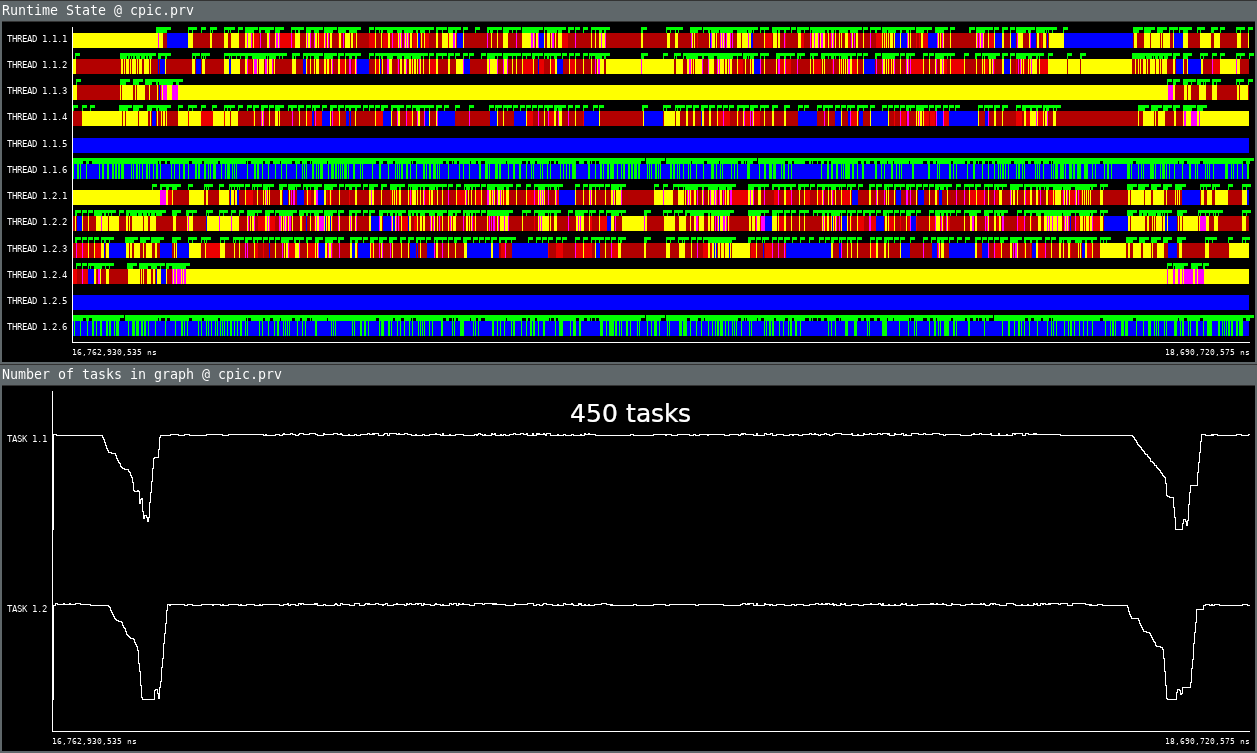
\includegraphics[width=0.95\linewidth]{fftw-ompss2.png}
	\caption{Tasks created inside the FFTW when using OmpSs-2: Up to 450 tasks are 
	created in rapid succession, with only 4 CPUs and 2 processes.}
	\label{fig:fftw-ompss2}
\end{figure}

In order to avoid a scalability problem, another approach was tested: Add 
support for OmpSs-2~in the FFTW to enable multithreading, following the same 
structure as OpenMP. The results obtained were similar as with the pthread case, 
but more insight was gained in how the task were created. It shown that the 
overhead added by the large amount of created and destructed quick tasks 
outweight any benefit that could be gained by multithreading.


We can mitigate the effect of the scaling by increasing the number of processes.  
In order to evaluate which ratio of processes and CPUs yields the best 
performance several configurations are tested. With a fixed number of maximum 
CPUs available set to 32, we increase the number of processes while we reduce 
the CPUs per process.


\begin{figure}[h]
	\centering
		\begin{tikzpicture}
		\begin{axis} [
			legend pos=outer north east,
			xmode=log,
			log basis x=2,
			xticklabels={0,1,2,4,8,16},
%			xticklabel style={
%			/pgf/number format/precision=3,
%			/pgf/number format/fixed},
			grid=major,
			xlabel=Number of CPUs per process,
			ylabel=Time per iteration (s),
			width=0.5\textwidth]
		\addplot [ybar stacked, fill=red!30!white] table [
			x index = {0},
			y index = {10},
			col sep=space] {csv/constant-cpus.csv};
		\addlegendentry{Solver}
		\addplot [ybar stacked, fill=blue!30!white] table [
			x index = {0},
			y index = {11},
			col sep=space] {csv/constant-cpus.csv};
		\addlegendentry{Particles}
		\addplot [only marks,error bars/y dir=both, error bars/y explicit] table [
			x index = {0},
			y index = {5},
			y error index={6},
			col sep=space] {csv/constant-cpus.csv};
		\addlegendentry{Total}
		\end{axis}
		\end{tikzpicture}
	\caption{The number of CPUs per process is incremented while reducing the 
	number of processes (the total number of CPUs is set to 32 and is kept 
	constant).  The time per iteration is measured, which leads to a 
	characteristic U shape.}
\end{figure}



